\documentclass{beamer}

%% Use package ----------------------------------------------------------------
\usepackage[T1]{fontenc}
\usepackage[utf8]{inputenc}
\usepackage{lmodern}
\usepackage{graphicx}
\usepackage[absolute,overlay]{textpos}
\usepackage{multicol}
\usepackage{listings}
\usepackage{svg}

%% Beamer customization--------------------------------------------------------

\usepackage{xcolor}
\usetheme{Warsaw}

%% Themes
% Outer themes
\useoutertheme{shadow}
% Rounded boxes and shadows
\useinnertheme[shadow=true]{rounded}
% Solid \item symbols
\useinnertheme{circles}

%% Custom colors
\definecolor{rltgreen}{rgb}{0,0.5,0}
\definecolor{pasteur}{RGB}{0,90,154}
\setbeamerfont{block title}{size={}}
\setbeamercolor{structure}{fg=pasteur}
\setbeamercolor{item}{fg=pasteur}

%Color of title
\setbeamertemplate{frametitle}
{
    \nointerlineskip
    \begin{beamercolorbox}[sep=0.3cm,ht=1.8em,wd=\paperwidth]{frametitle}
        \vbox{}\vskip-2ex%
        \strut\insertframetitle\strut
        \vskip-0.8ex%
    \end{beamercolorbox}
}
% Hide navigation symbols
\setbeamertemplate{navigation symbols}{}

%% Title block
\setbeamercolor*{title}{use=structure,fg=white,bg=pasteur}

\makeatletter

%% Top infolines
\setbeamertemplate{headline}{%
\leavevmode%
  \hbox{%
    \begin{beamercolorbox}[wd=\paperwidth,ht=2.5ex,dp=1.125ex]{palette quaternary}%
    \insertsectionnavigationhorizontal{\paperwidth}{}{\hskip0pt plus1filll}
    \end{beamercolorbox}%
  }
}

%% Define Snakemake -----------------------------------------------------------

\definecolor{eclipseBlue}{RGB}{42,0.0,255}
\definecolor{eclipseGreen}{RGB}{63,127,95}
\definecolor{eclipsePurple}{RGB}{127,0,85}

\lstset{language=Python}
\lstset{
    basicstyle=\scriptsize\ttfamily,
    morekeywords={rule, output, shell, params, run, configfile, temp, log},
    showstringspaces=false,
    commentstyle=\color{eclipseGreen}, % style of comments
    keywordstyle=\color{eclipsePurple}, % style of keywords
    stringstyle=\color{eclipseBlue}, % style of strings
}


%% Set up title ---------------------------------------------------------------

\title[Sequana]{Sequana: a set of flexible genomic pipelines for processing and reporting NGS analysis}
\author[D.Desvillechabrol]{Dimitri Desvillechabrol}
\institute{Institut Pasteur}
\date{Dec 12th 2016, Institut Pasteur}



\AtBeginSection[]{
  \begin{frame}
  \vfill
  \centering
  \begin{beamercolorbox}[sep=8pt,center,shadow=true,rounded=true]{title}
    \usebeamerfont{title}\insertsectionhead\par%
  \end{beamercolorbox}
  \vfill
  \end{frame}
}

\begin{document}

%% Title slide ----------------------------------------------------------------

\begin{frame}[plain]
    \titlepage
    \begin{textblock*}{5cm}(4.5cm,0.3cm)
        
\includegraphics[scale=0.09]{images/Institut_Pasteur.png}
    \end{textblock*}
\end{frame}

%% Slides ---------------------------------------------------------------------

\section{Motivation}

\begin{frame}
    \frametitle{NGS at Biomics (Sean Kennedy)}
 
 Development driven by the Biomics Pole at Pasteur Institute, which involves
 many aspects of NGS including :
 
 \tiny
 \begin{block}{https://research.pasteur.fr/en/team/biomics/}
  \begin{itemize}
  \item De novo and targeted sequencing of viruses, prokaryotes and eukaryotes
  \item Variant (SNP, indel, large rearrangements) detection
  \item Human and Mouse SNP detection by array
  \item Transcriptional analysis (RNA-Seq) for both prokaryotes and eukaryotes
  \item 16S and deep-sequencing metagenomic studies (mouse, human, and other environments)
  \item Bottom-up whole proteomic analysis and quantification
  \item Analysis of a wide range of post-translational modifications
  \item Determination of the dynamics of protein complexes.
  \item Epigenetics (CHIP-Seq, methylation studies)
  \item Projects involving two or more techniques (i.e. proteogenomics, single-cell DNA/RNA analysis)
  \end{itemize}
 \end{block}
 \small 
\end{frame}

\section{Pipelines}

\begin{frame}{Pipelines available in Sequana}
    \begin{textblock*}{5cm}(0.3cm,1.3cm)
        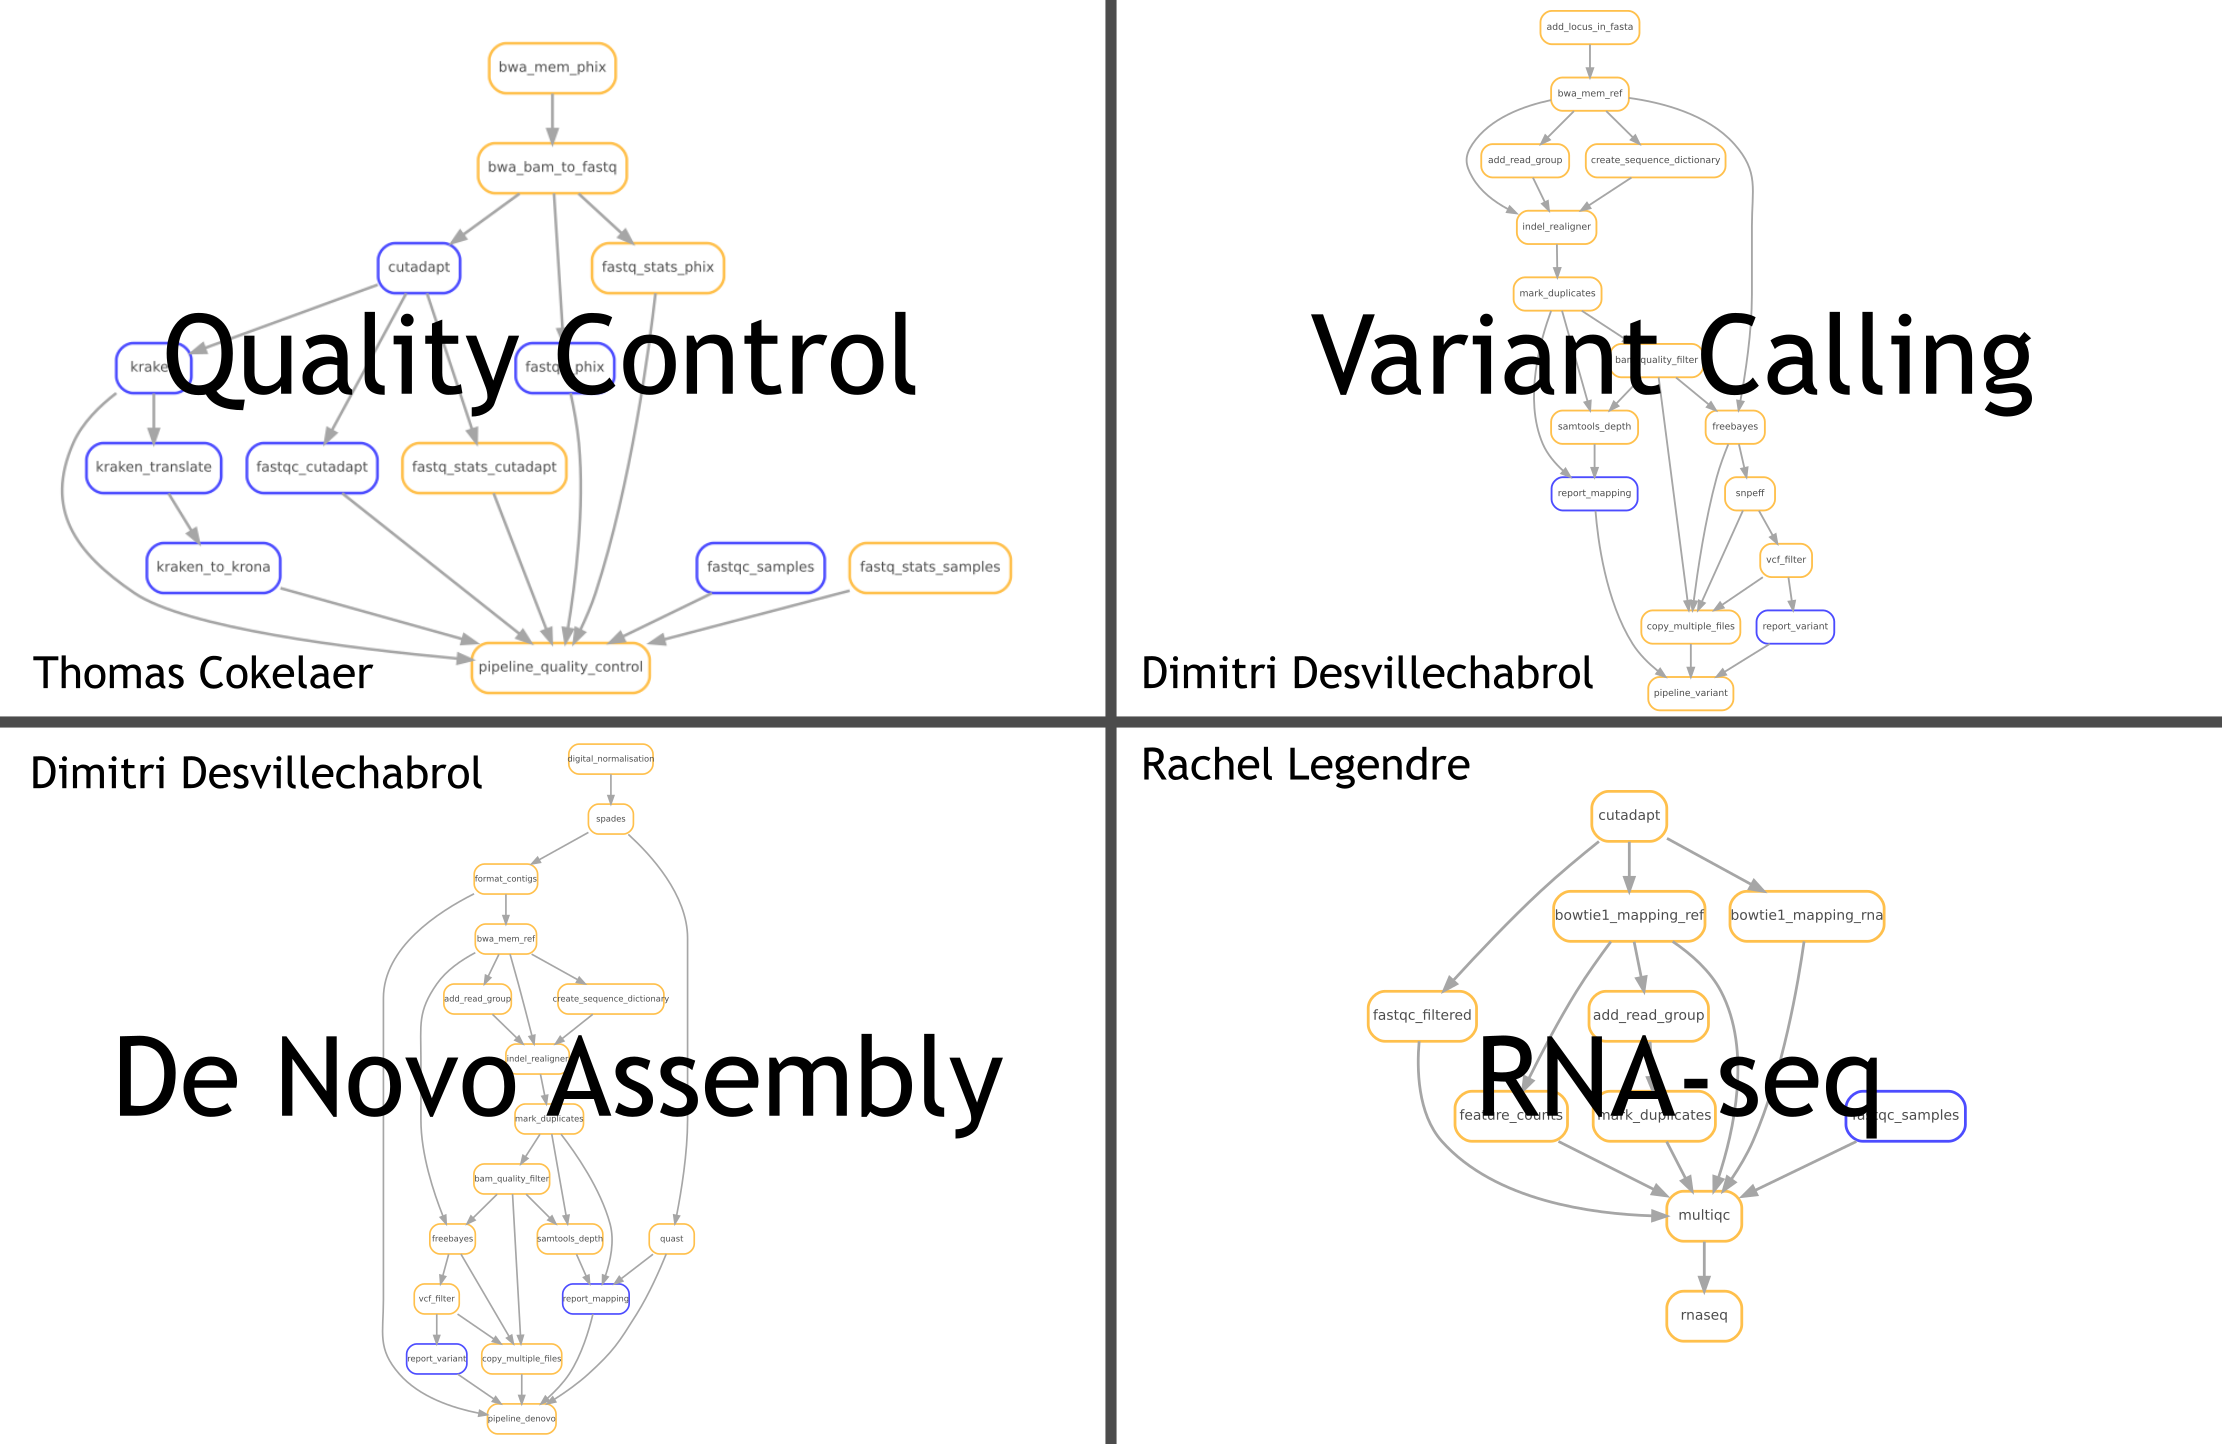
\includegraphics[scale=0.215]{images/pipelines}
    \end{textblock*}
\end{frame}

\begin{frame}[fragile]{Rules specificity: input and output are variables}
    \begin{itemize}
        \item Rules are generic and easily reusable
        \begin{block}{mark\_duplicates.rules}
        \begin{lstlisting}
rule mark_duplicates:
    input:
        __mark_duplicates__input
    output:
        bam = __mark_duplicates__output,
        metrics = __mark_duplicates__metrics
    log:
        out = __mark_duplicates__log_std,
        err = __mark_duplicates__log_err
        \end{lstlisting}
        \end{block}
    \end{itemize}
\end{frame}

\begin{frame}[fragile]{Dynamics rules}
    \begin{itemize}
        \item Each rule must be unique in a pipeline
        \begin{alertblock}{}
        Some pipelines must use multiple times one rules like fastqc in quality control pipeline
        \end{alertblock}
        \item These rules are templatized to become dynamic:
        \begin{block}{quality\_control.rules}
        \begin{lstlisting}
exec(open(sequana.modules["fastqc"], "r").read())
        ...
include: fastqc_dynamic("samples", manager)
        ...
include: fastqc_dynamic("phix", manager)
        ...
include: fastqc_dynamic(adapter_removal, manager)
        \end{lstlisting}
        \end{block}
    \end{itemize}
\end{frame}

\section{Usage}

\begin{frame}[fragile]{Using command line}
    \begin{itemize}
        \item One command line to initiate the pipeline
    \end{itemize}
    \begin{exampleblock}{Shell}
    \begin{lstlisting}[language={}]
    sequana --pipeline variant_calling \
            --input-directory path/to/sample/ \
            --reference sequence.fasta \
            --output-directory analysis/
    \end{lstlisting}
    \end{exampleblock}
    \begin{itemize}
        \item The sequana executable creates a directory with the project name
        \item The directory contains all the necessary files (config, snakefile)
    \end{itemize}
\end{frame}


\section{Continuous Integration}

\begin{frame}{Versioning, Test and Documentation}
\begin{itemize}
    \item Sequana is available on GitHub (github.com/sequana/sequana)
    \item Continuous Integration on Travis with 60 tests with 60\% coverage
    \item Documentation available on sequana.readthedocs.org~.
        \begin{itemize}
            \item Uses Sphinx (RST syntax) to document the source code and provides user guide.
            \item Updated automatically at each commits
        \end{itemize}
\end{itemize}
\end{frame}

\section{GUI}

\begin{frame}{GUI to simplify the usage of snakemake}
    \begin{columns}
        \begin{column}{0.5\textwidth}

            \only<1>{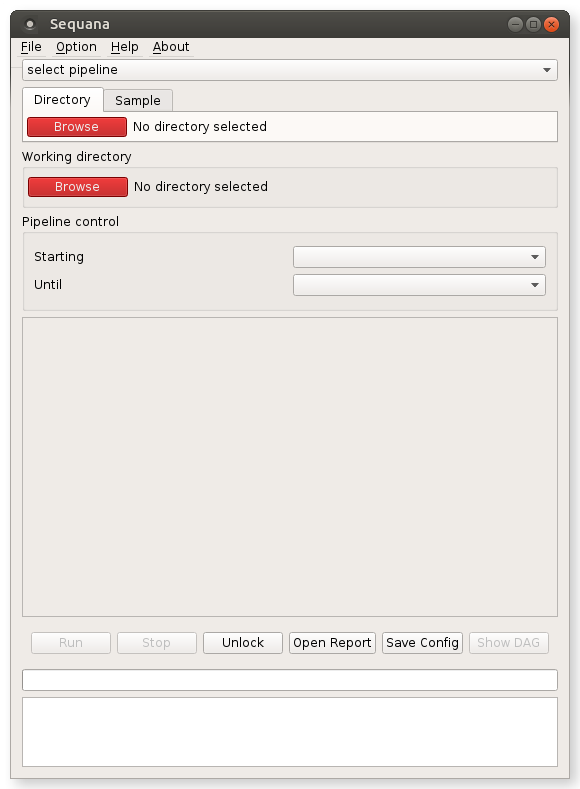
\includegraphics[scale=0.25]{images/sequana_init}}

            \only<2>{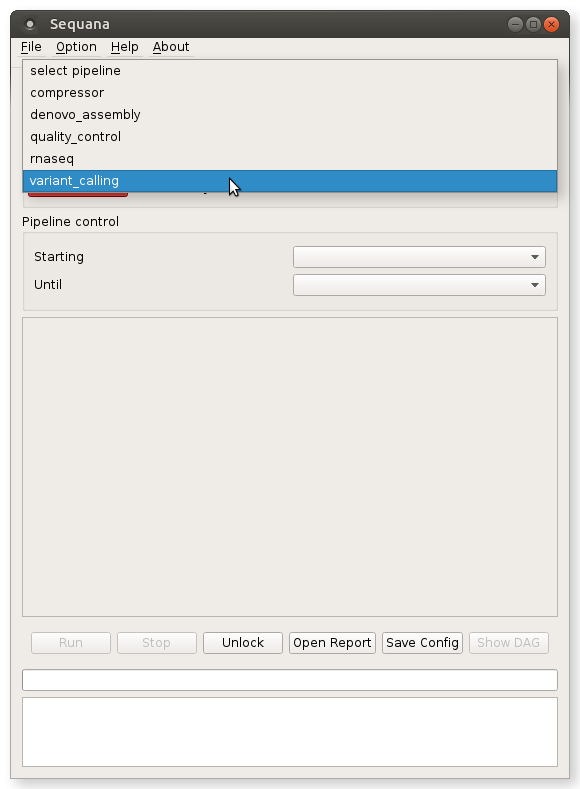
\includegraphics[scale=0.25]{images/choose_pipeline}}

            \only<3>{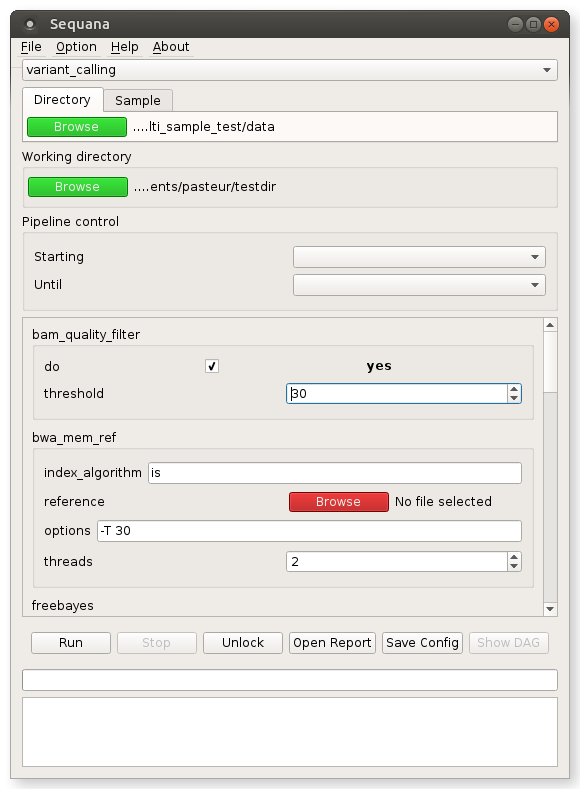
\includegraphics[scale=0.25]{images/choose_input_output}}

            \only<4>{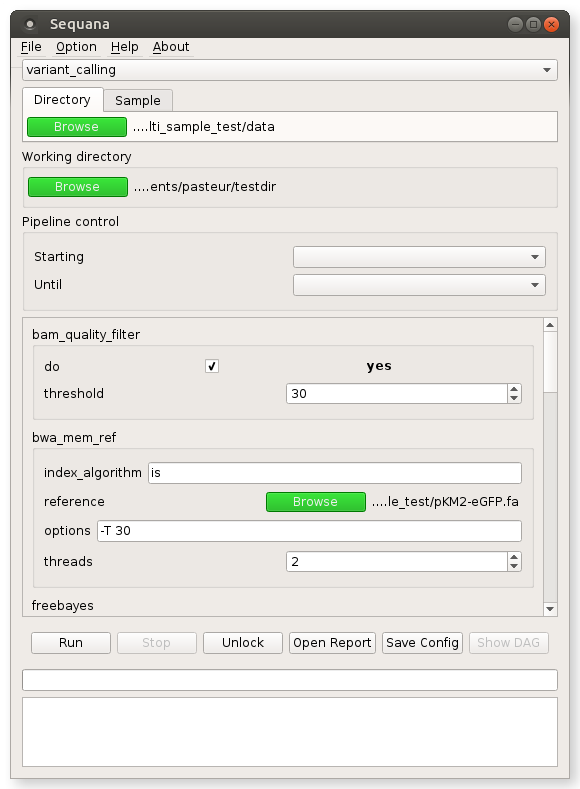
\includegraphics[scale=0.25]{images/sequana_pipeline}}

            \only<5>{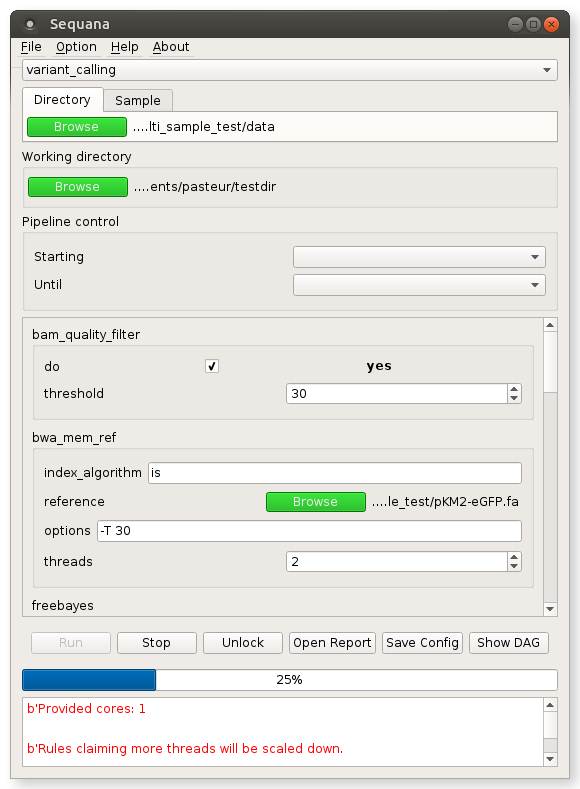
\includegraphics[scale=0.25]{images/sequana_running}}
            
            \only<6>{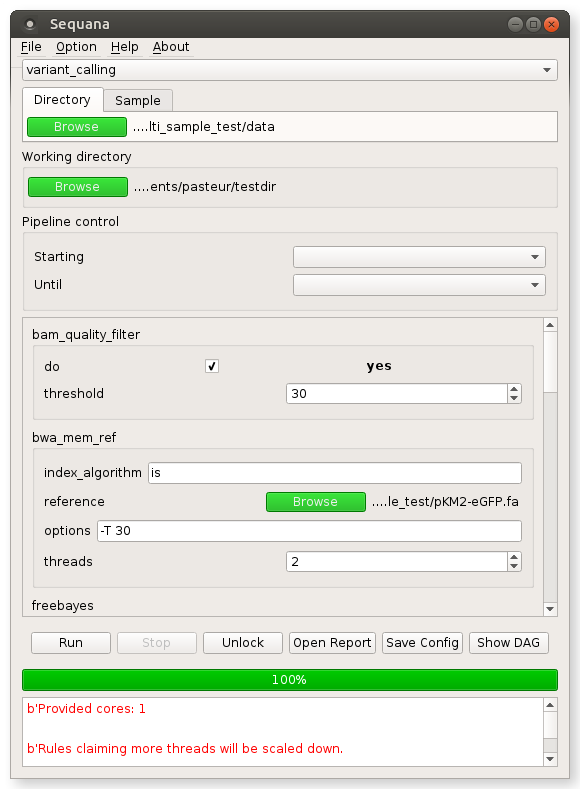
\includegraphics[scale=0.25]{images/sequana_finish}}

            \only<7>{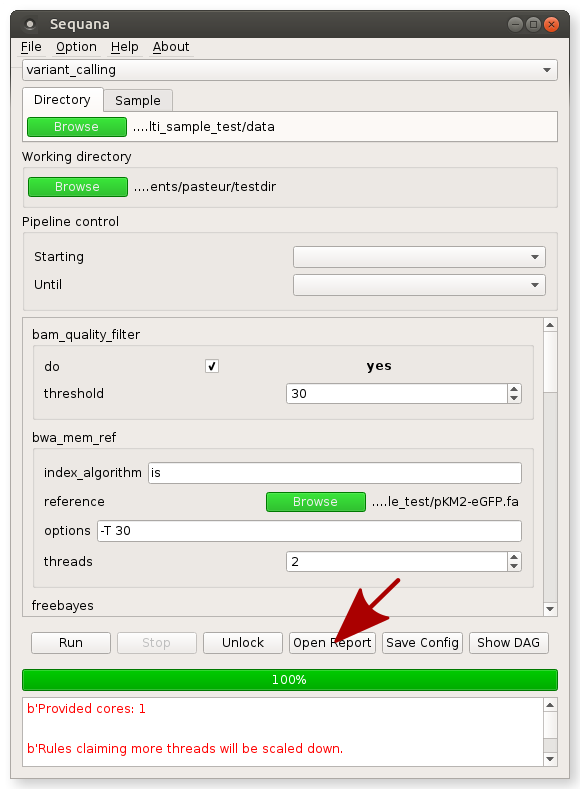
\includegraphics[scale=0.3125]{images/sequana_open_report}}

        \end{column}
        \begin{column}{0.5\textwidth}
            \only<1>{
                \begin{itemize}
                    \item Interface developed with PyQT5 and python
                    \item Wrap our snakemake pipelines to ease the usage
                    \item Usable on our cluster, which allows X11
                \end{itemize}
            }
            \only<2-6>{
            \begin{enumerate}
                \item<2-6> Choose a pipeline
                \item<3-6> Set input and output
                \item<4-6> Fill the config formular
                \item<5-6> Run the pipeline
                \item<6> Finished !
            \end{enumerate}
            }
            \only<7>{
                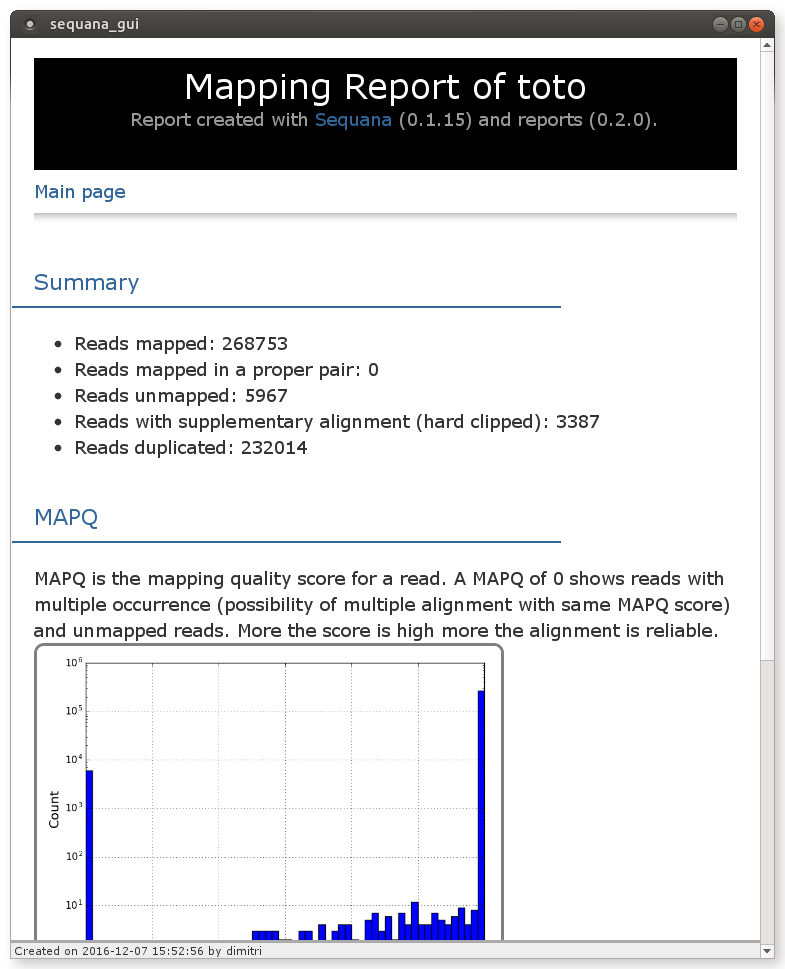
\includegraphics[scale=0.2]{images/report_toto}
            }
        \end{column}
    \end{columns}
\end{frame}

\begin{frame}{Ease the pipeline manipulation and viewing}
    \begin{columns}
        \begin{column}{0.5\textwidth}

            \only<1>{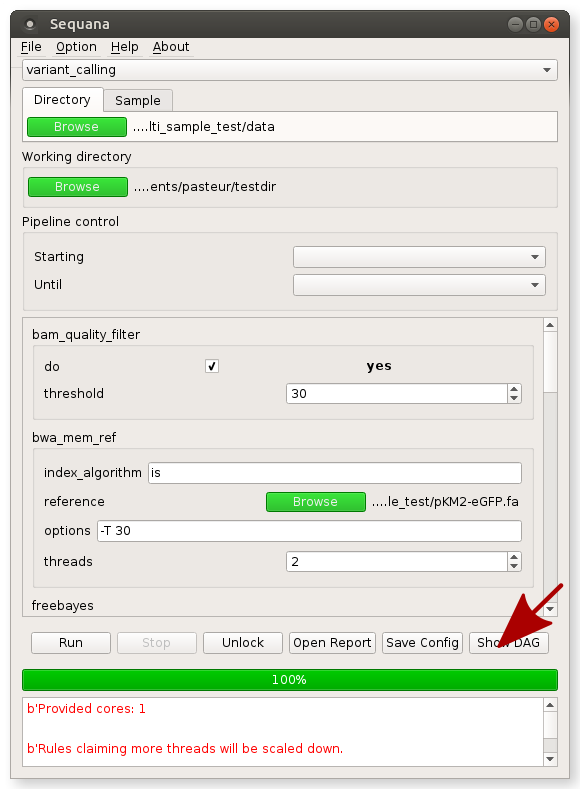
\includegraphics[scale=0.3125]{images/sequana_show_dag}}

            \only<2>{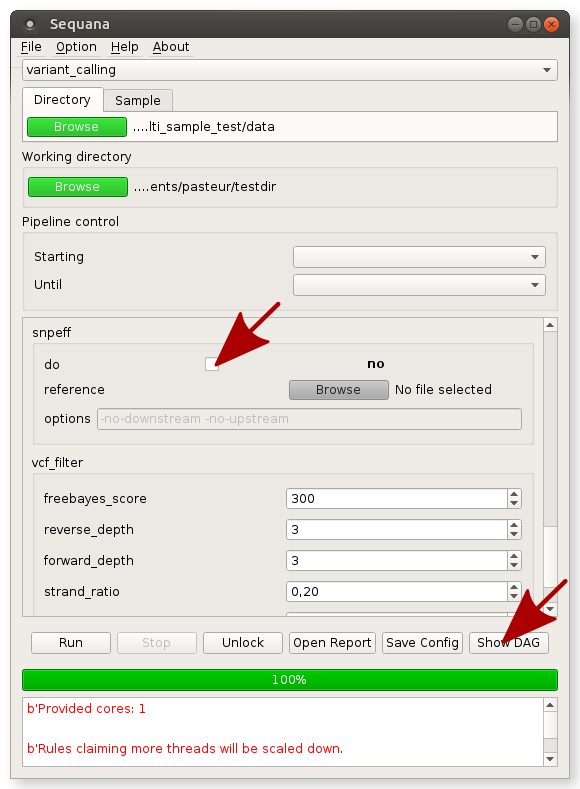
\includegraphics[scale=0.3125]{images/unactivate_snpeff}}

            \only<3>{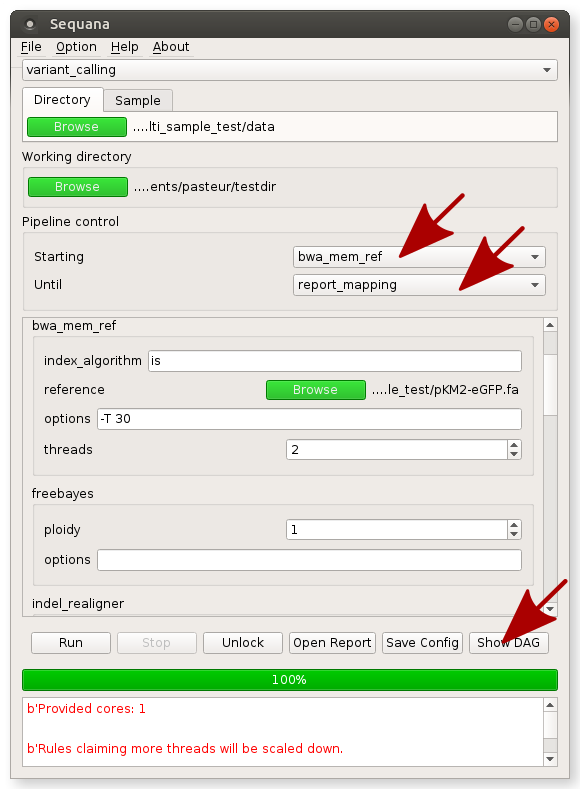
\includegraphics[scale=0.3125]{images/starting_until}}

        \end{column}
        \begin{column}{0.5\textwidth}

            \only<1>{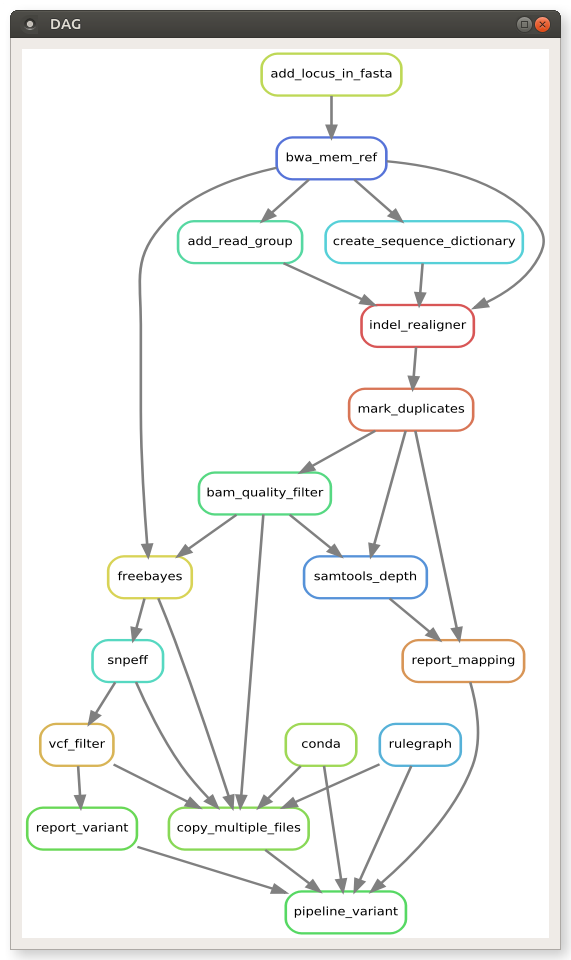
\includegraphics[scale=0.20]{images/full_dag}}

            \only<2>{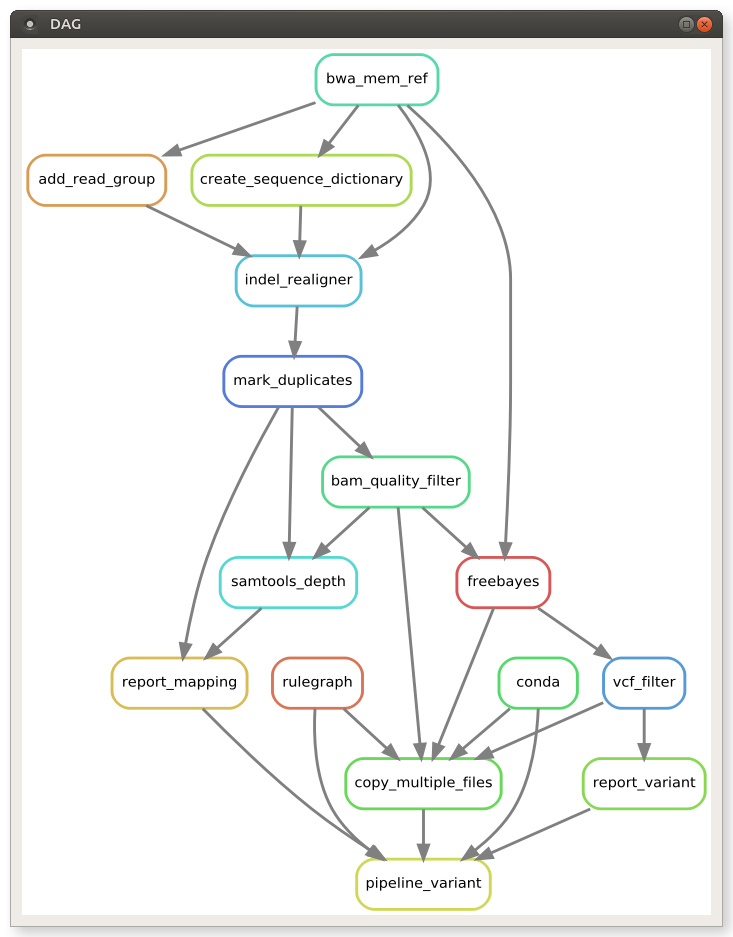
\includegraphics[scale=0.21]{images/dag_without_snpeff}}

            \only<3>{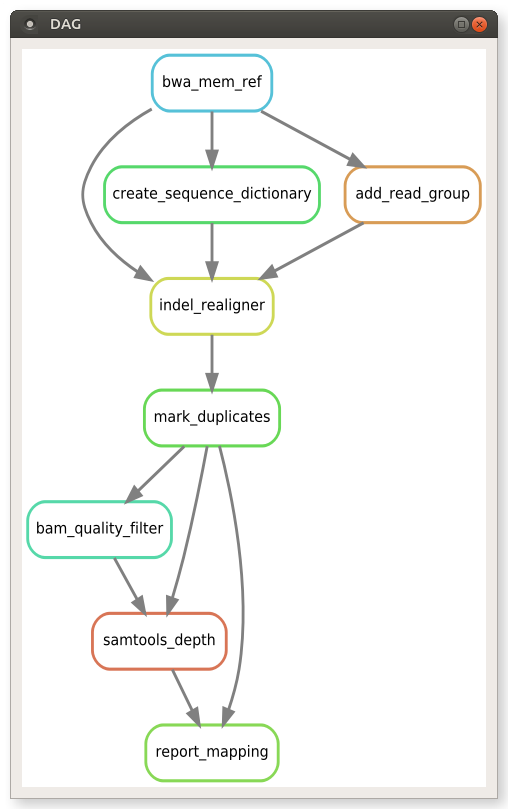
\includegraphics[scale=0.24]{images/dag_report_mapping}}

        \end{column}

    \end{columns}
\end{frame}

\section{Summary and Future Directions}

\begin{frame}{Sequana history}
    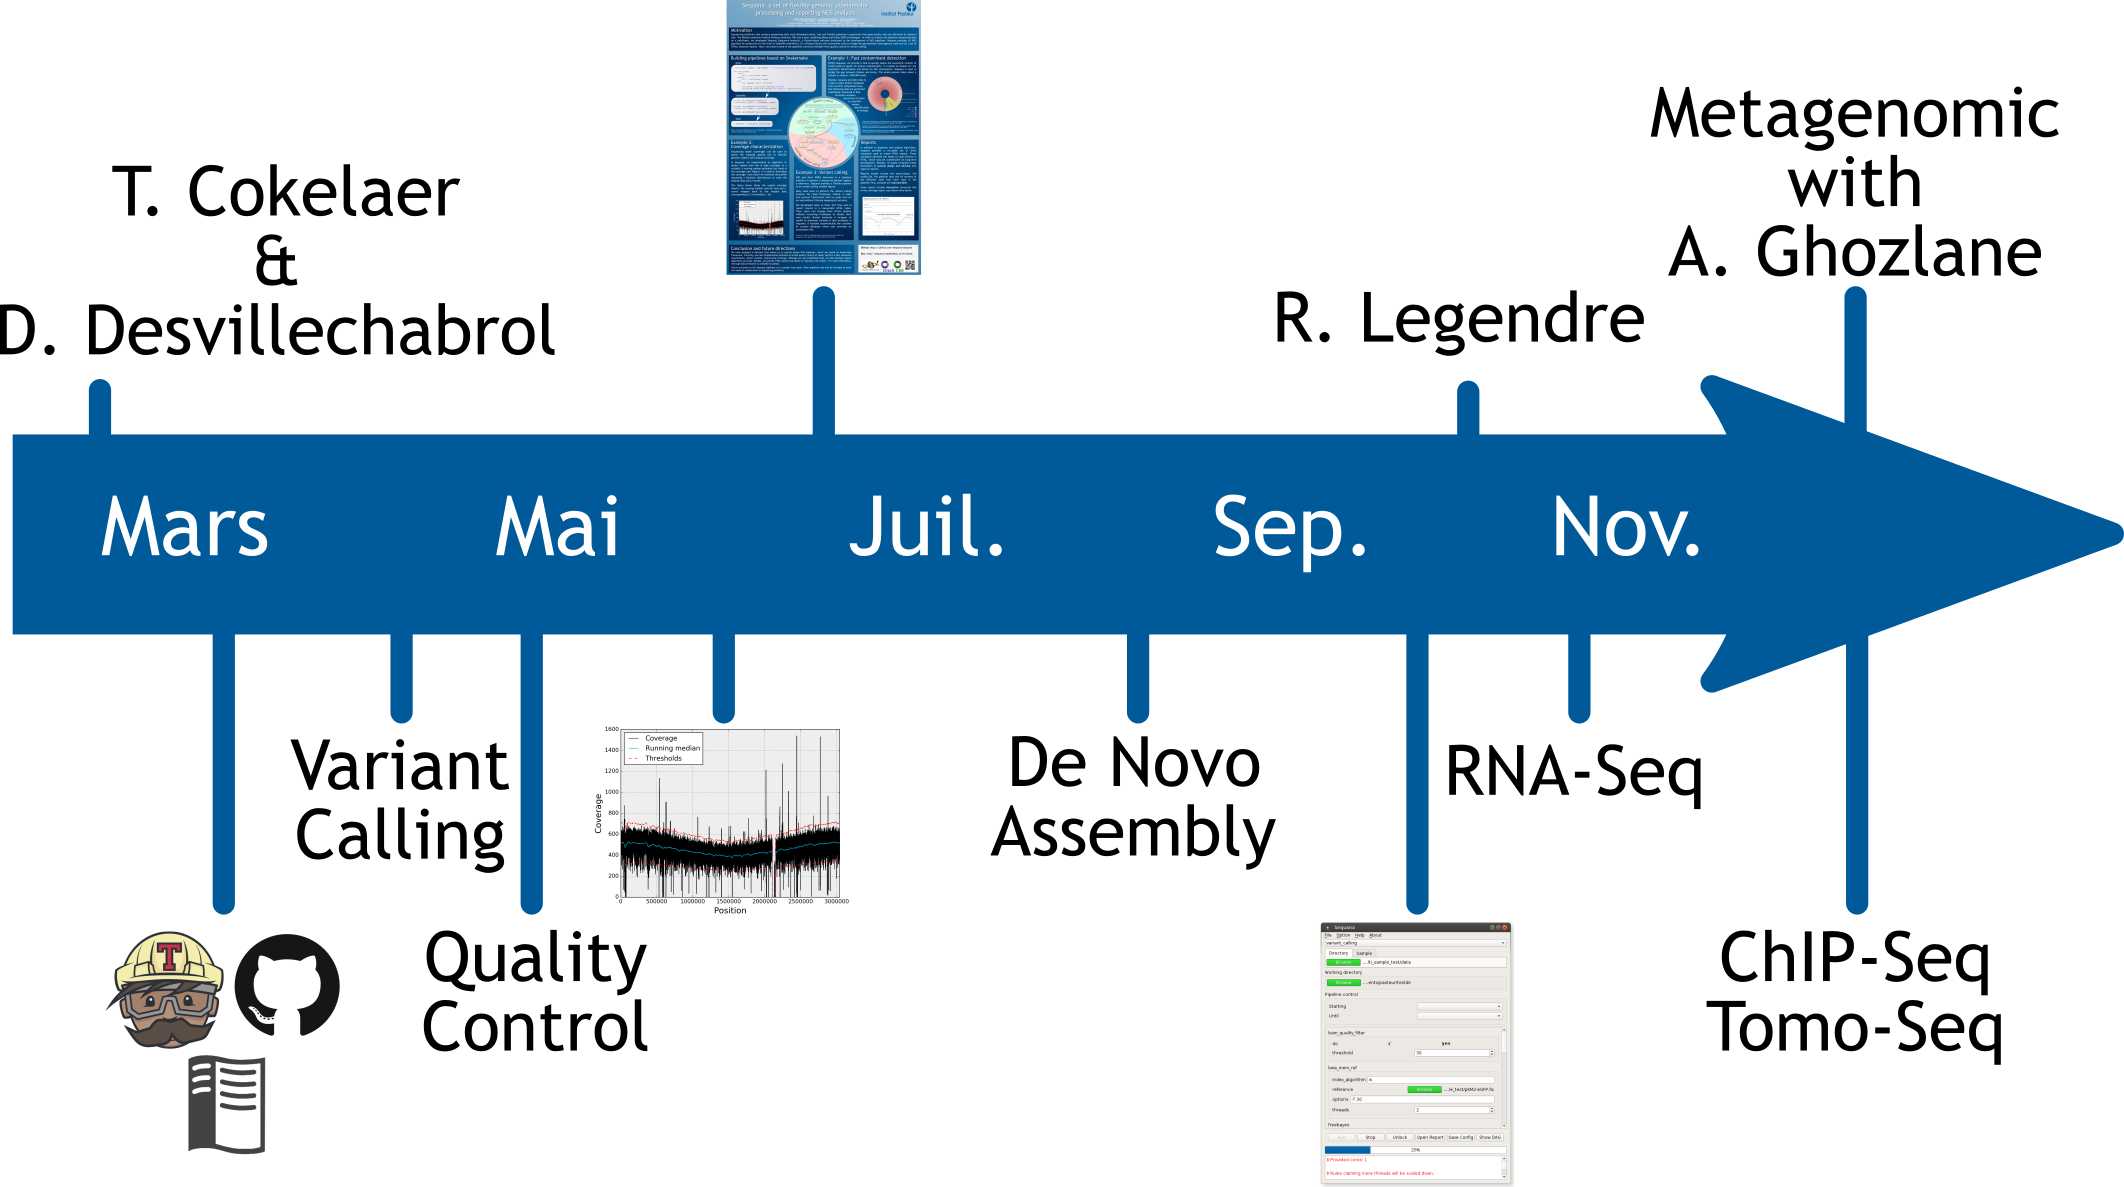
\includegraphics[scale=0.2]{images/timeline}
    \footnotetext[1]{\tiny Detection and characterization of low and high genome coverage regions using an efficient running median and a double threshold approach.
Dimitri Desvillechabrol, Christiane Bouchier, Sean Kennedy, Thomas Cokelaer
bioRxiv 092478; doi: http://dx.doi.org/10.1101/092478}
\end{frame}

\begin{frame}{Acknowledgement}
    \begin{columns}[t]
        \begin{column}{0.5\textwidth}
            \begin{itemize}
                \item Developers:
                \begin{itemize}
                    \item Thomas Cokelaer
                    \item Rachel Legendre
                \end{itemize}
                \item Beta-tester:
                    \begin{itemize}
                        \item Christiane Bouchier
                    \end{itemize}
                \item Fruitful discussions:
                    \begin{itemize}
                        \item Claudia Chica
                        \item Varun Khanna
                        \item Pierre Lechat
                        \item Frédéric Lemoine
                        \item Hervé Ménager
                        \item Bioinformatics and Biostatistics HUB 
                    \end{itemize}
            \end{itemize}
        \end{column}
        \begin{column}{0.5\textwidth}
            \begin{itemize}
                \item Biomics team:
                \begin{itemize}
                    \item Jean-Yves Copee
                    \item Amine Ghozlane
                    \item Sean Kennedy
                    \item Béatrice Regnault
                    \item Hugo Varet
                \end{itemize}
                \item Organizations:

                    
\includegraphics[scale=0.07]{images/citech}

                    
\includegraphics[scale=0.18,trim=0 8cm 0 9cm,clip]{images/france_genomique}
            \end{itemize}
        \end{column}
    \end{columns}
\end{frame}

\end{document}
